%! TEX program = xelatex
\documentclass[tikz]{standalone}
\usepackage[lining]{ebgaramond}
\usepackage[math-style=ISO, bold-style=ISO]{unicode-math}
\setmathfont{Garamond-Math.otf}
\begin{document}
  \begin{tikzpicture}
    \node[align=left]{%
      \includegraphics[height=5.5cm]{muon-veto.jpg}%
      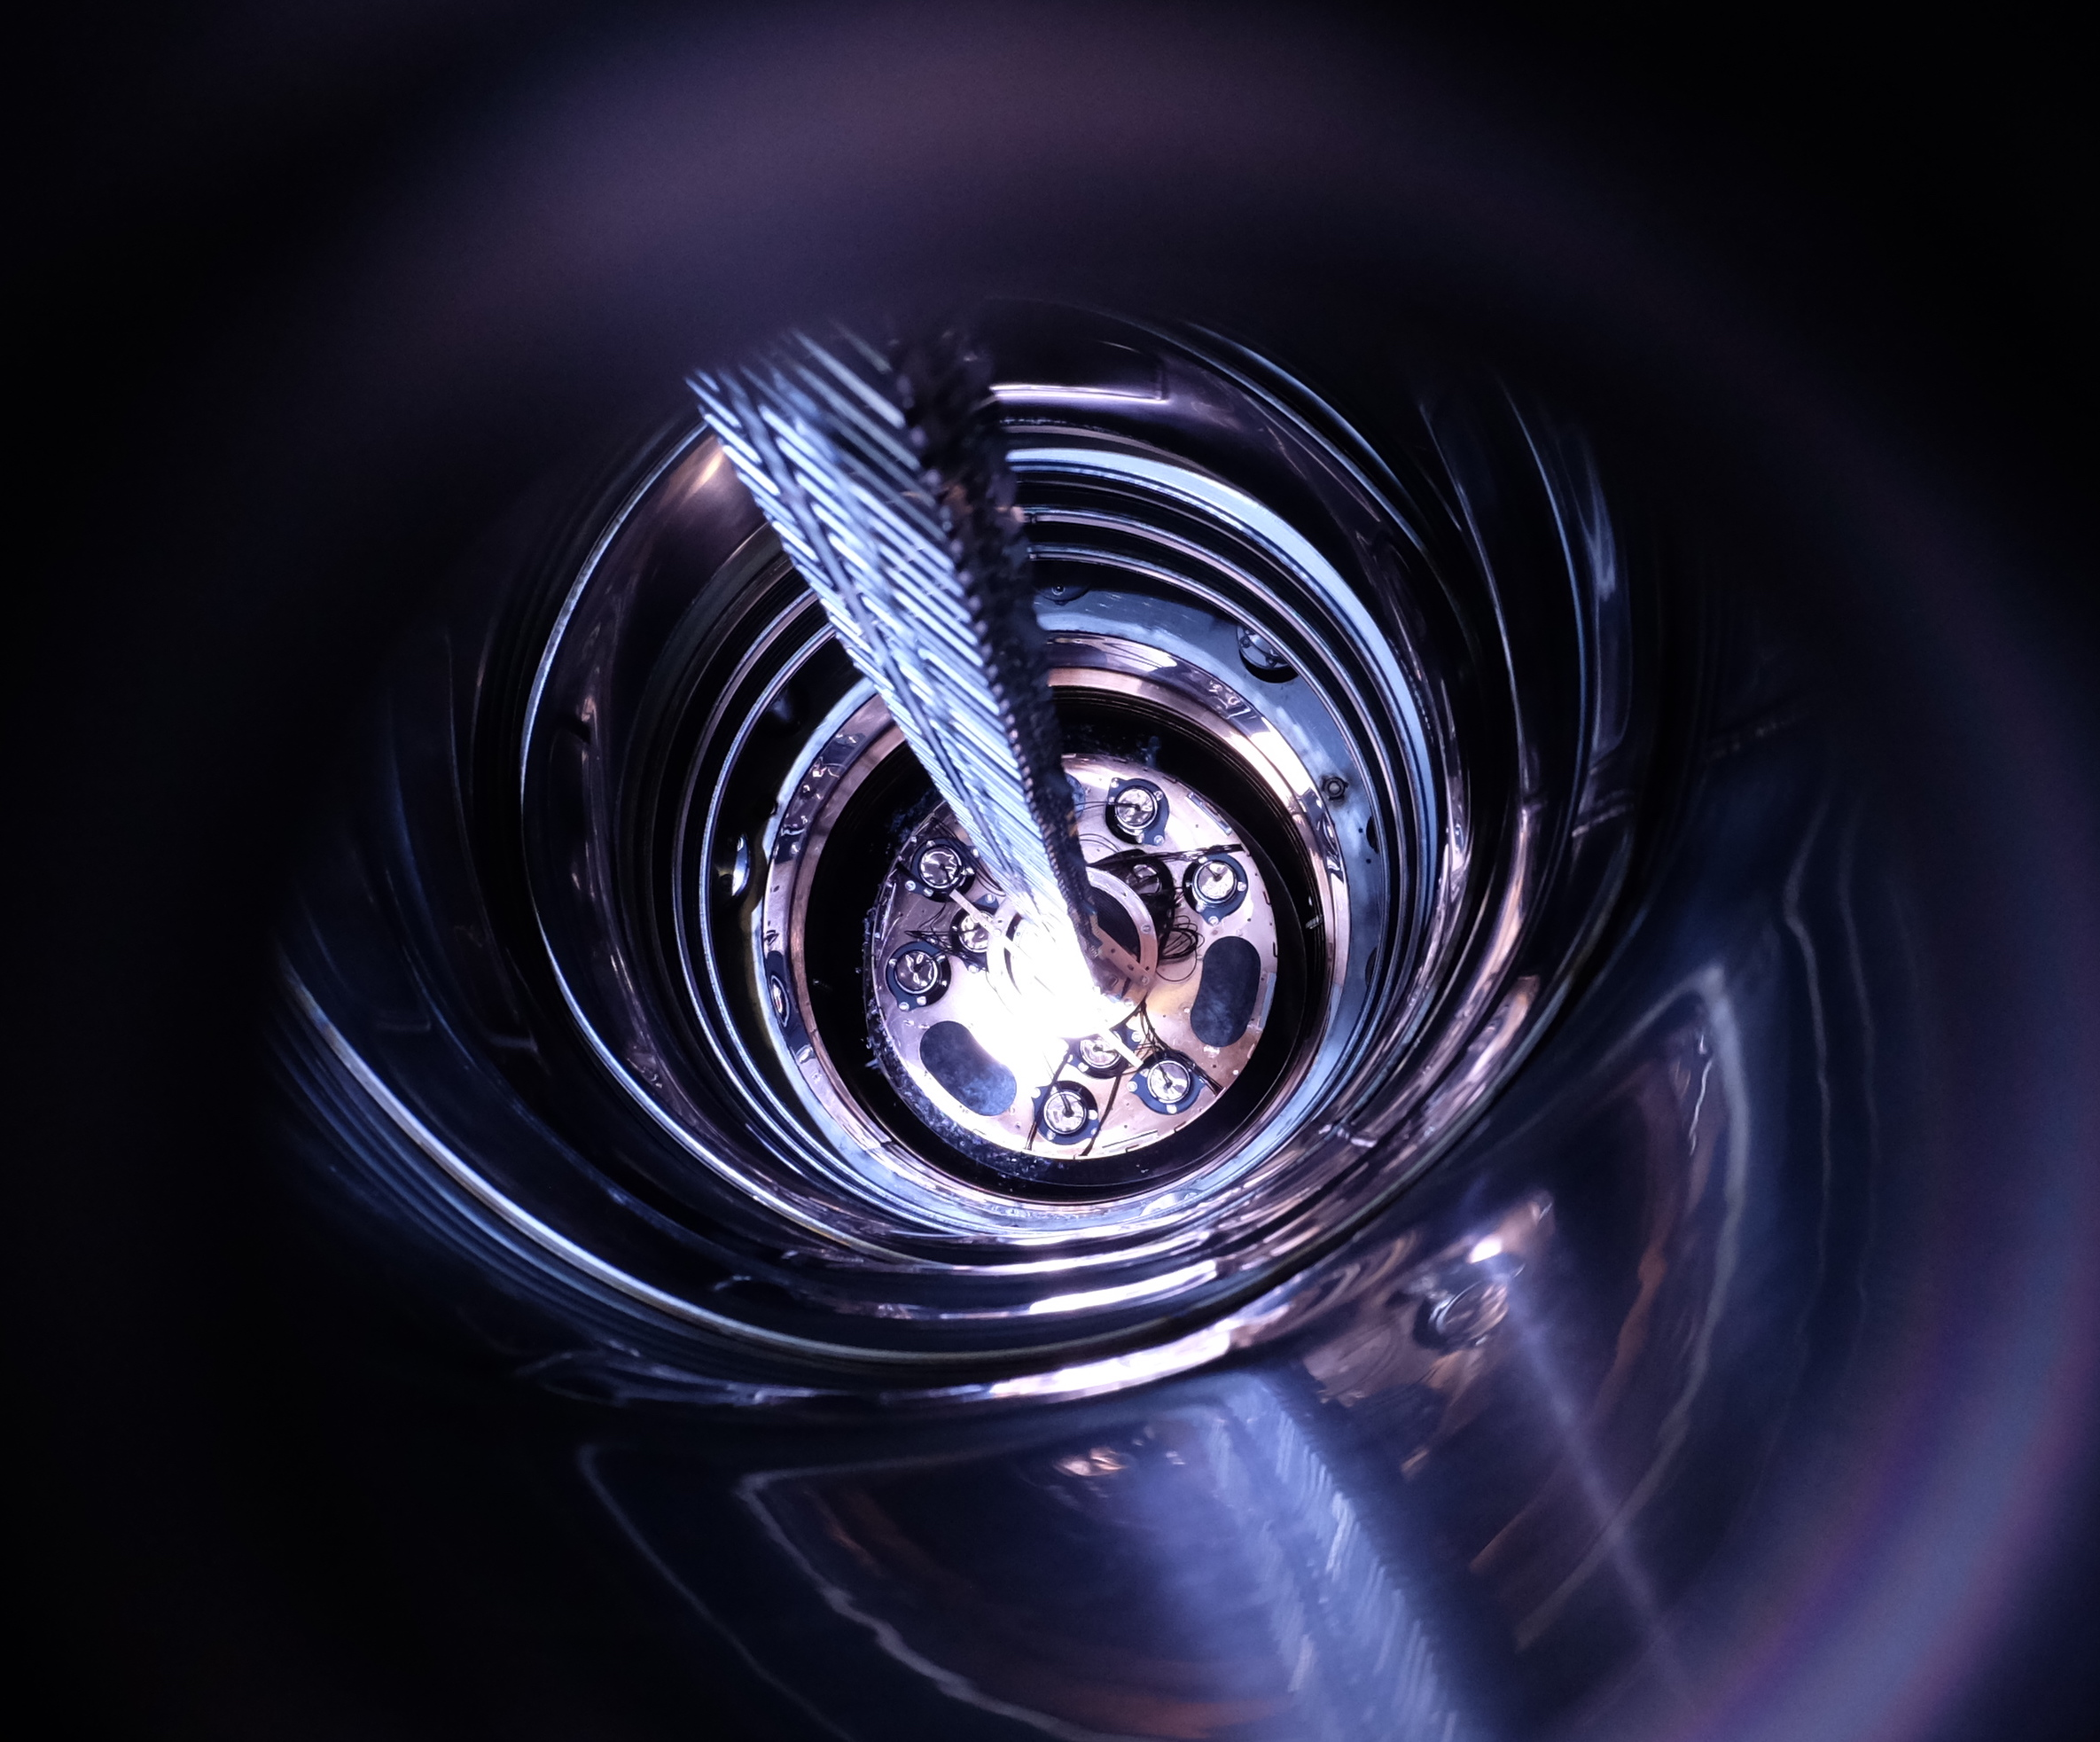
\includegraphics[height=5.5cm]{array-lowering.jpg}\\%
      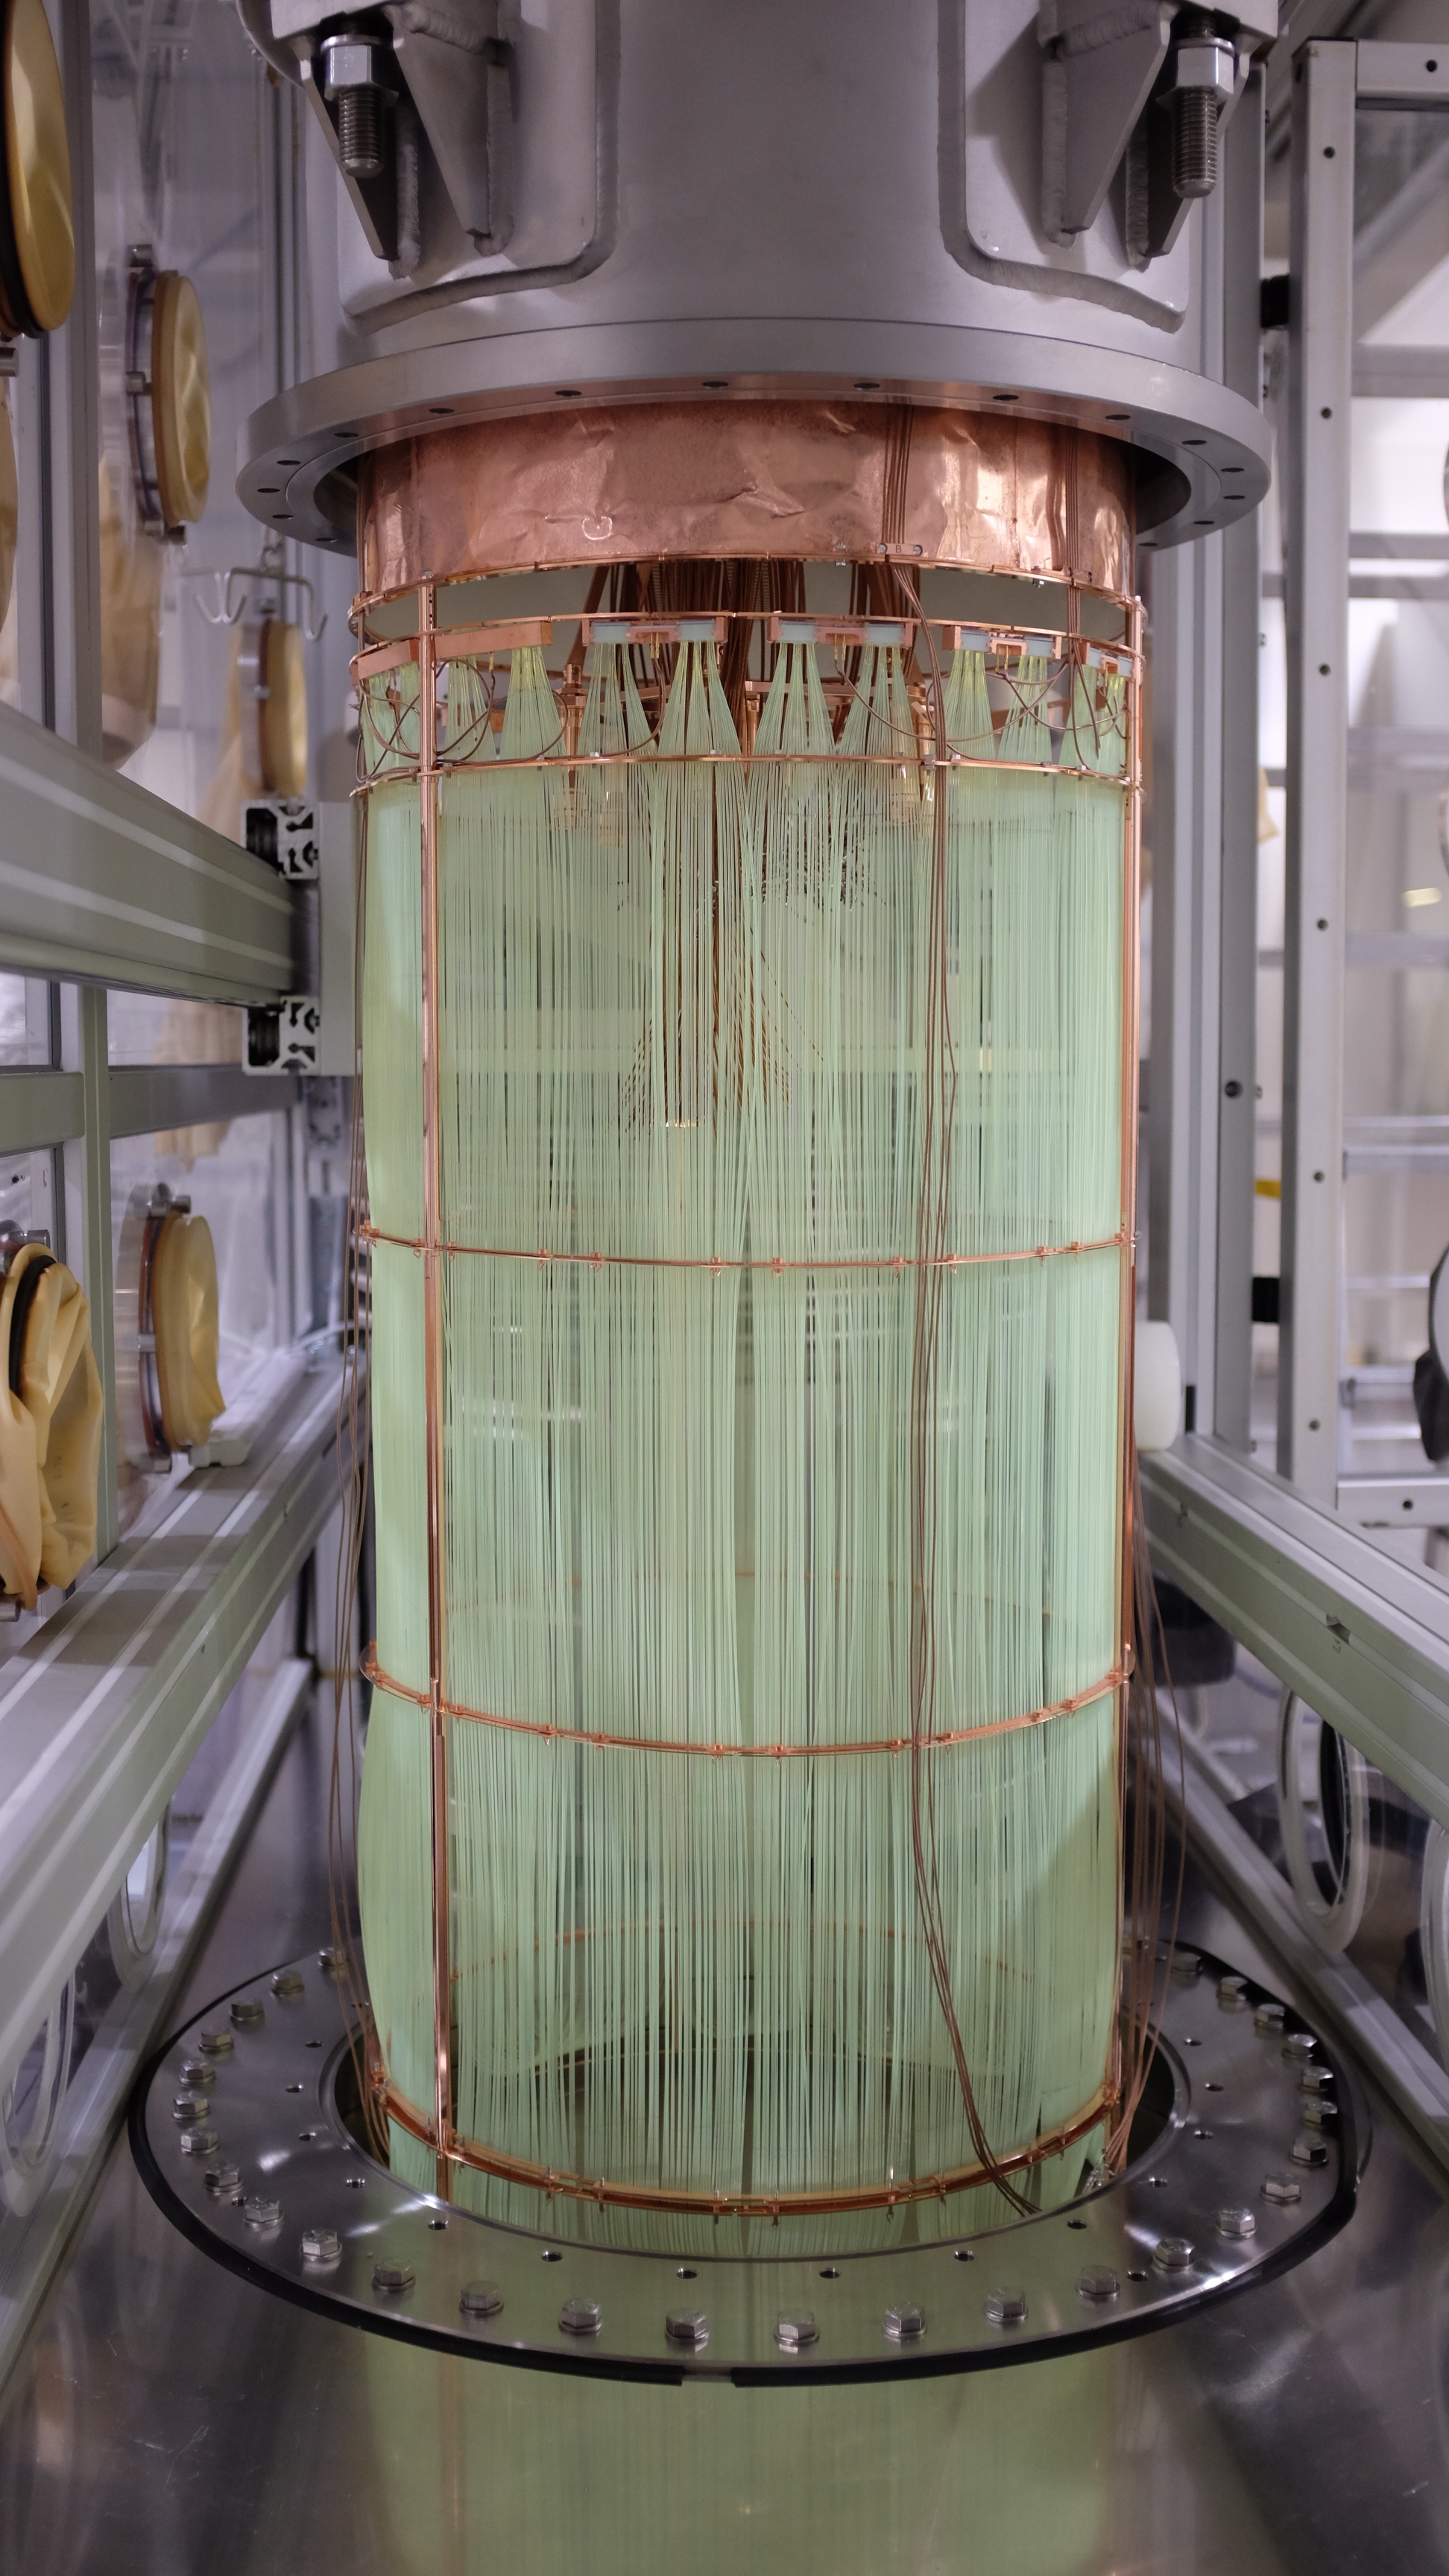
\includegraphics[height=7.2cm]{fiber-shroud.jpg}%
      \includegraphics[height=7.2cm]{strings1.jpg}%
      \includegraphics[height=7.2cm]{strings2.jpg}\\
      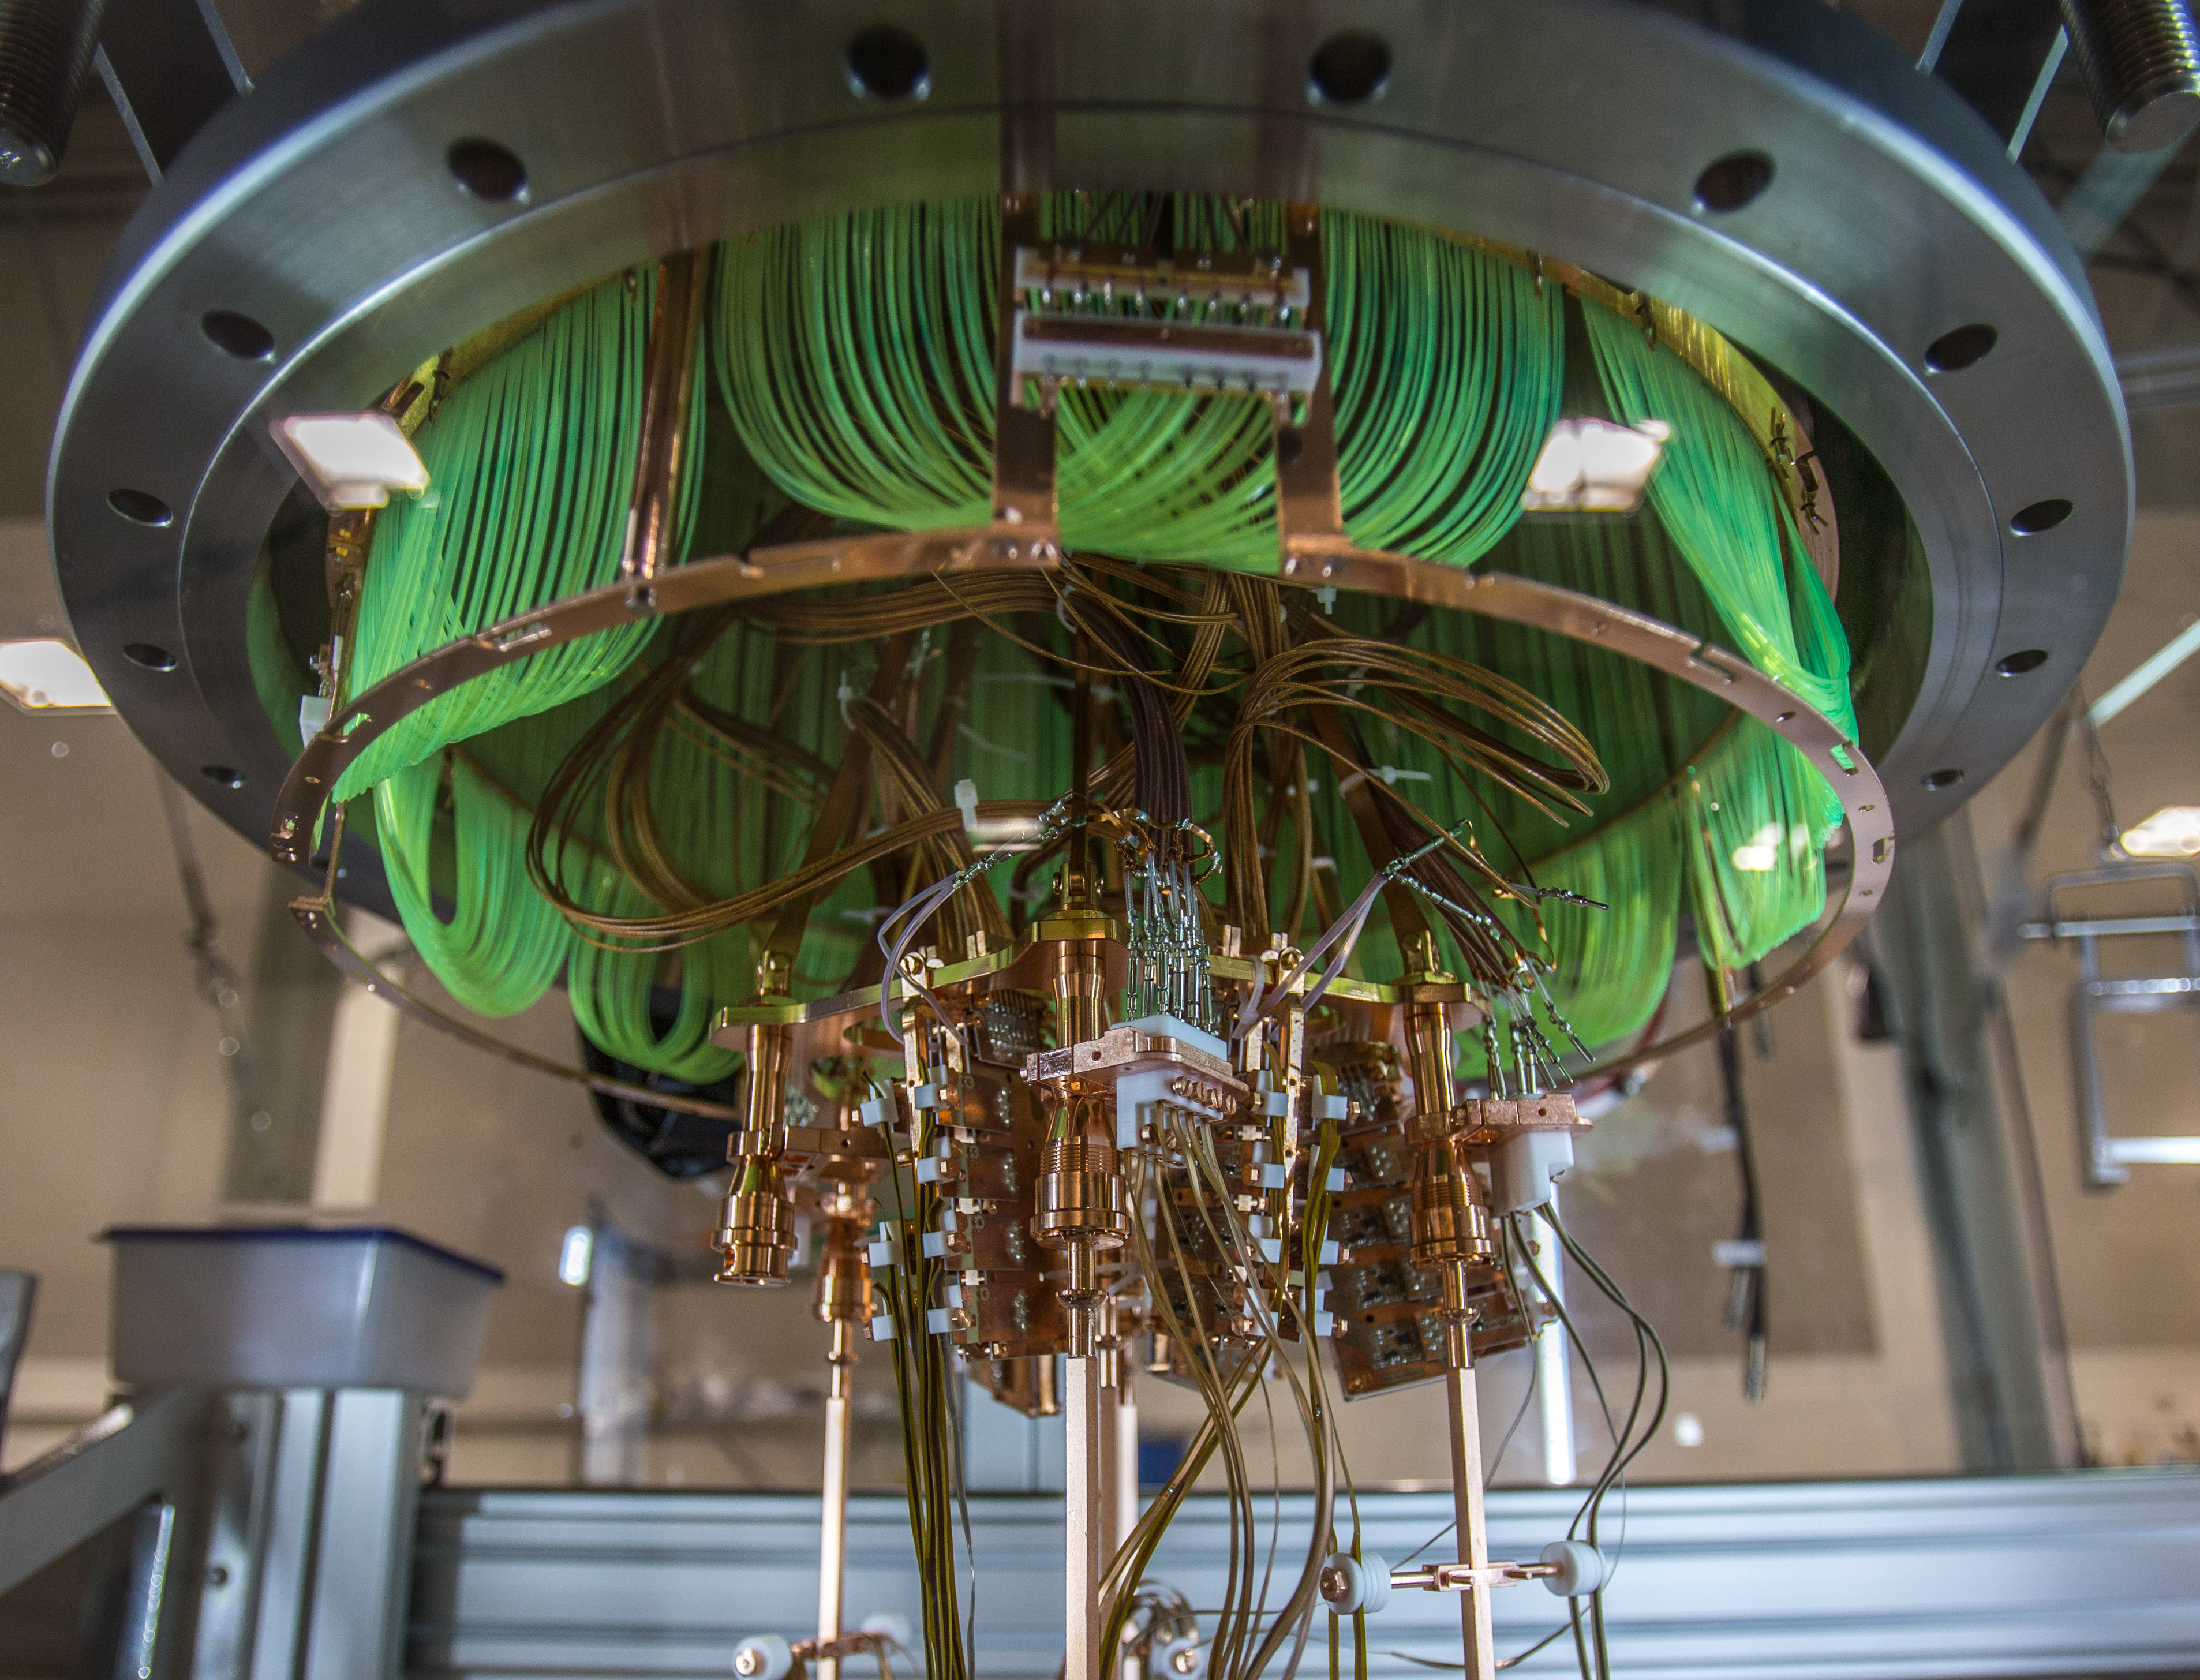
\includegraphics[height=3.7cm]{electronics.jpg}%
      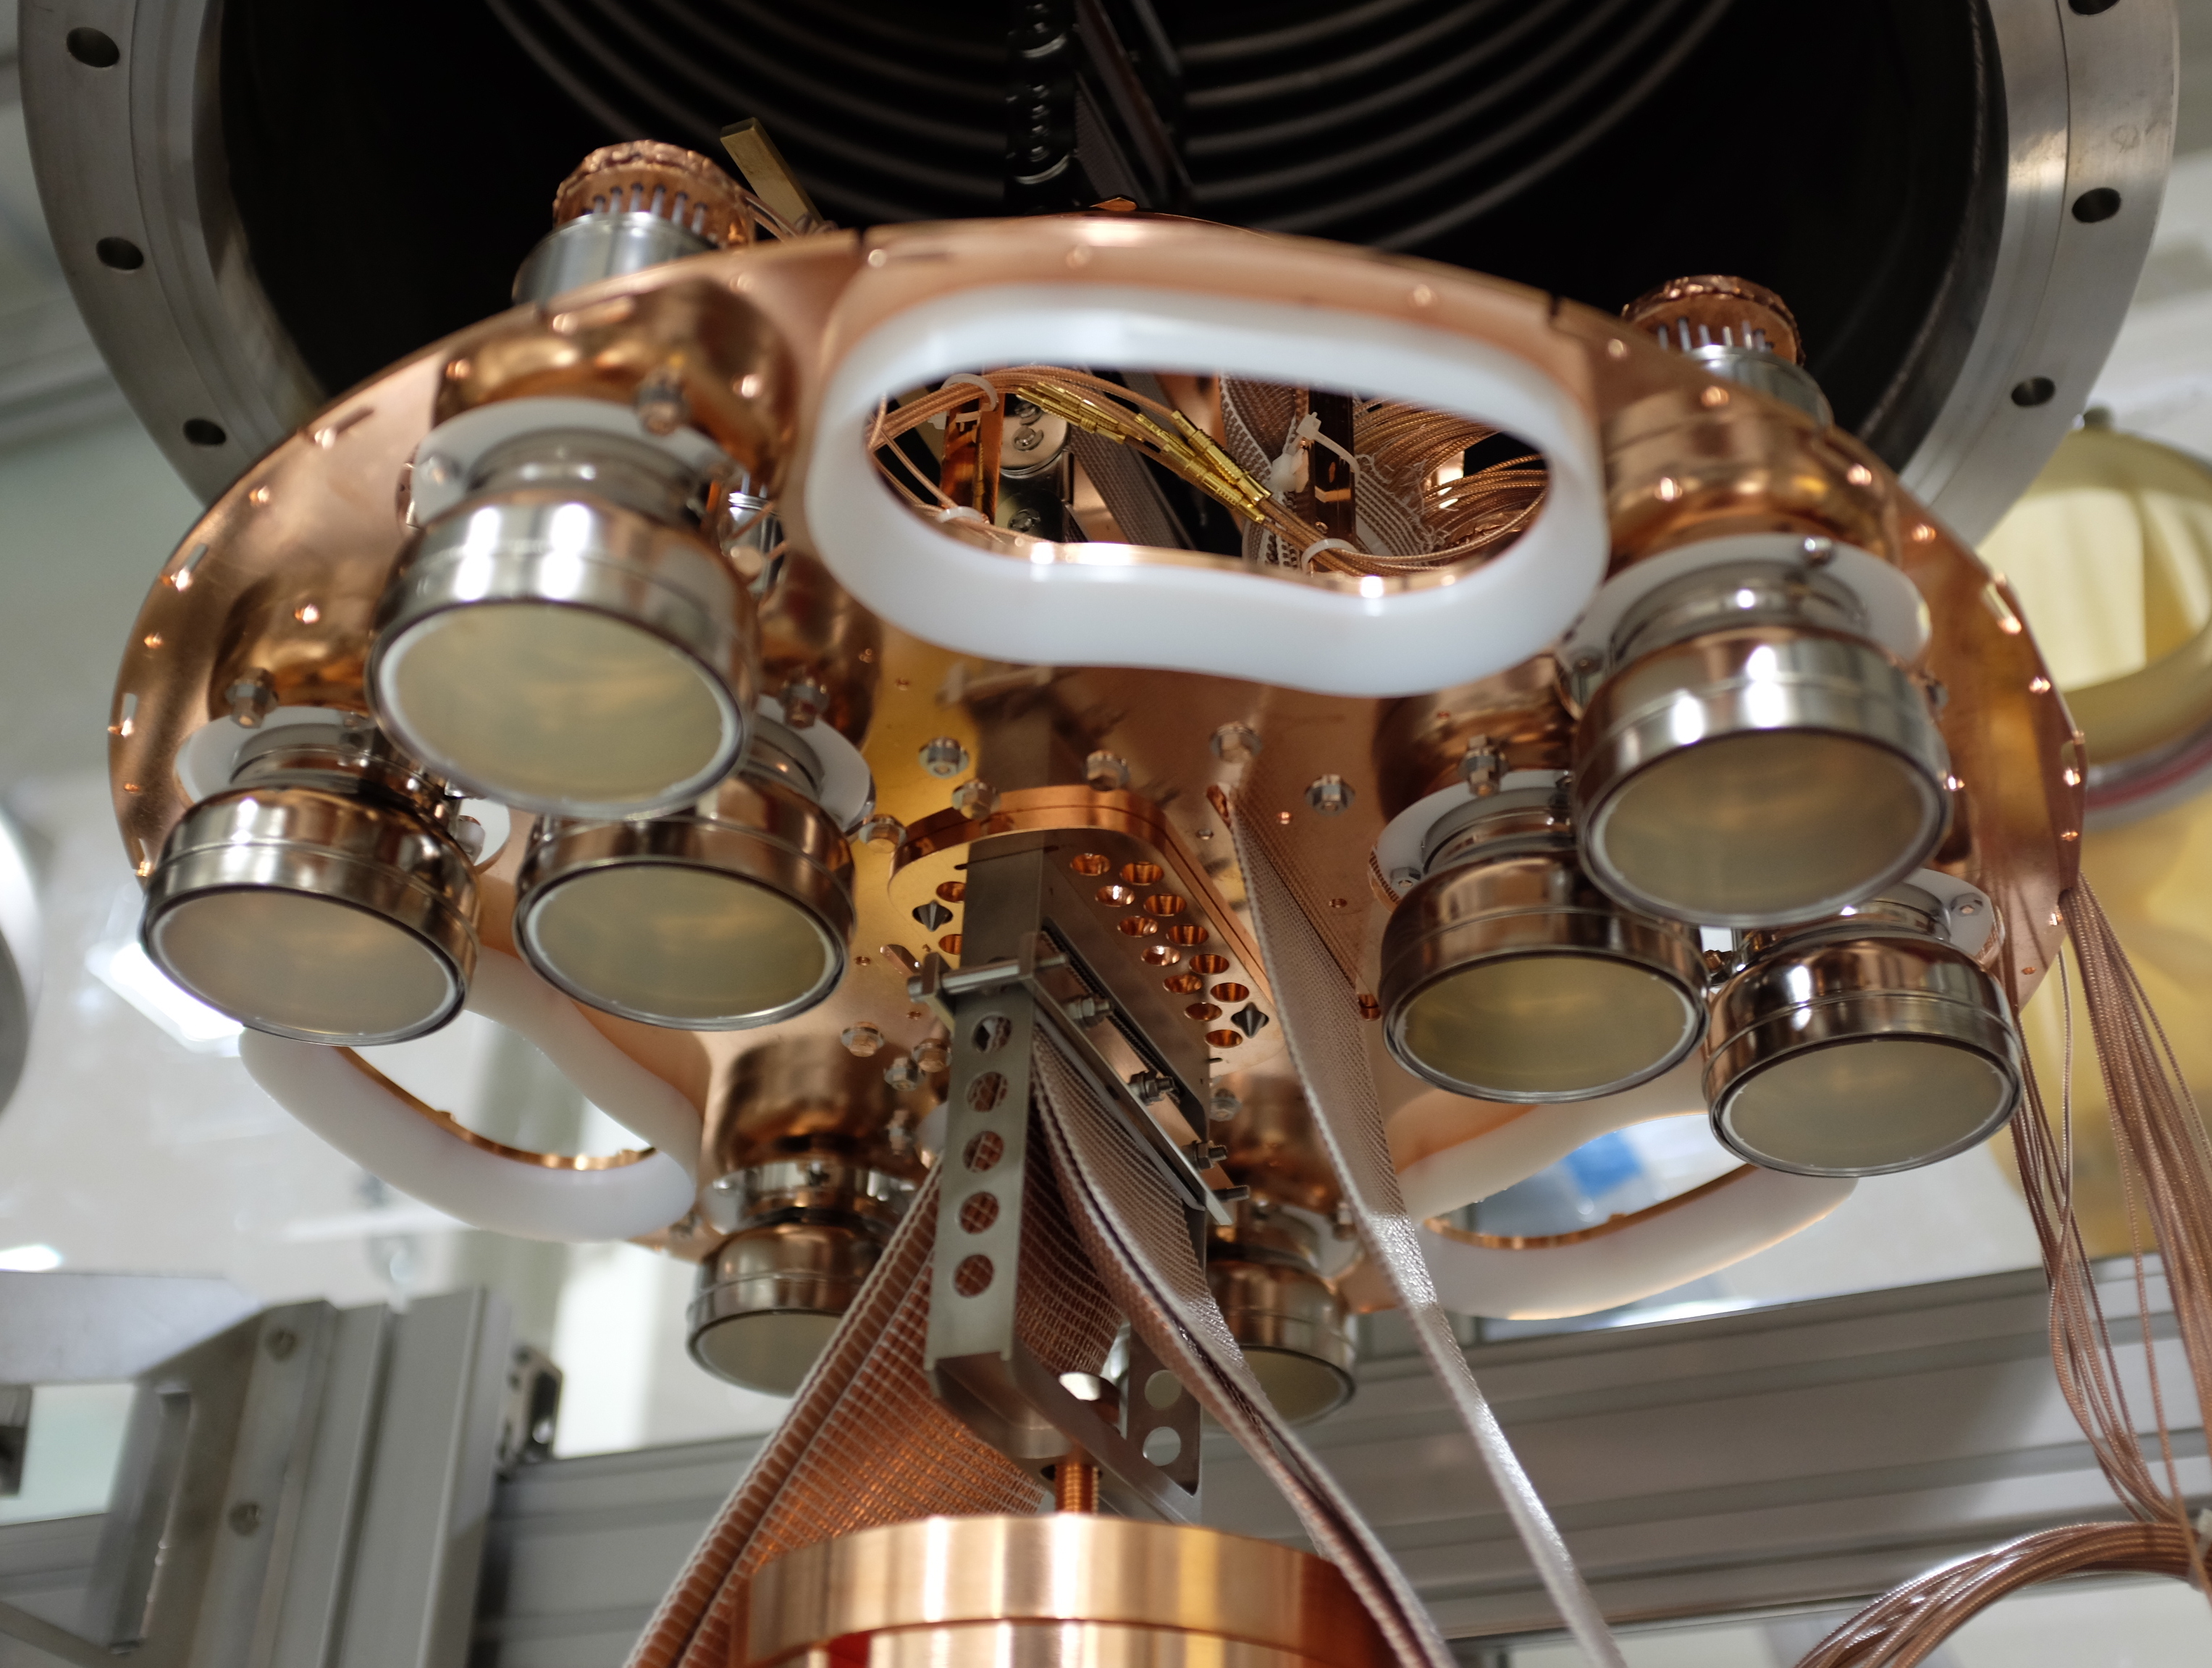
\includegraphics[height=3.7cm]{top-pmts.jpg}%
      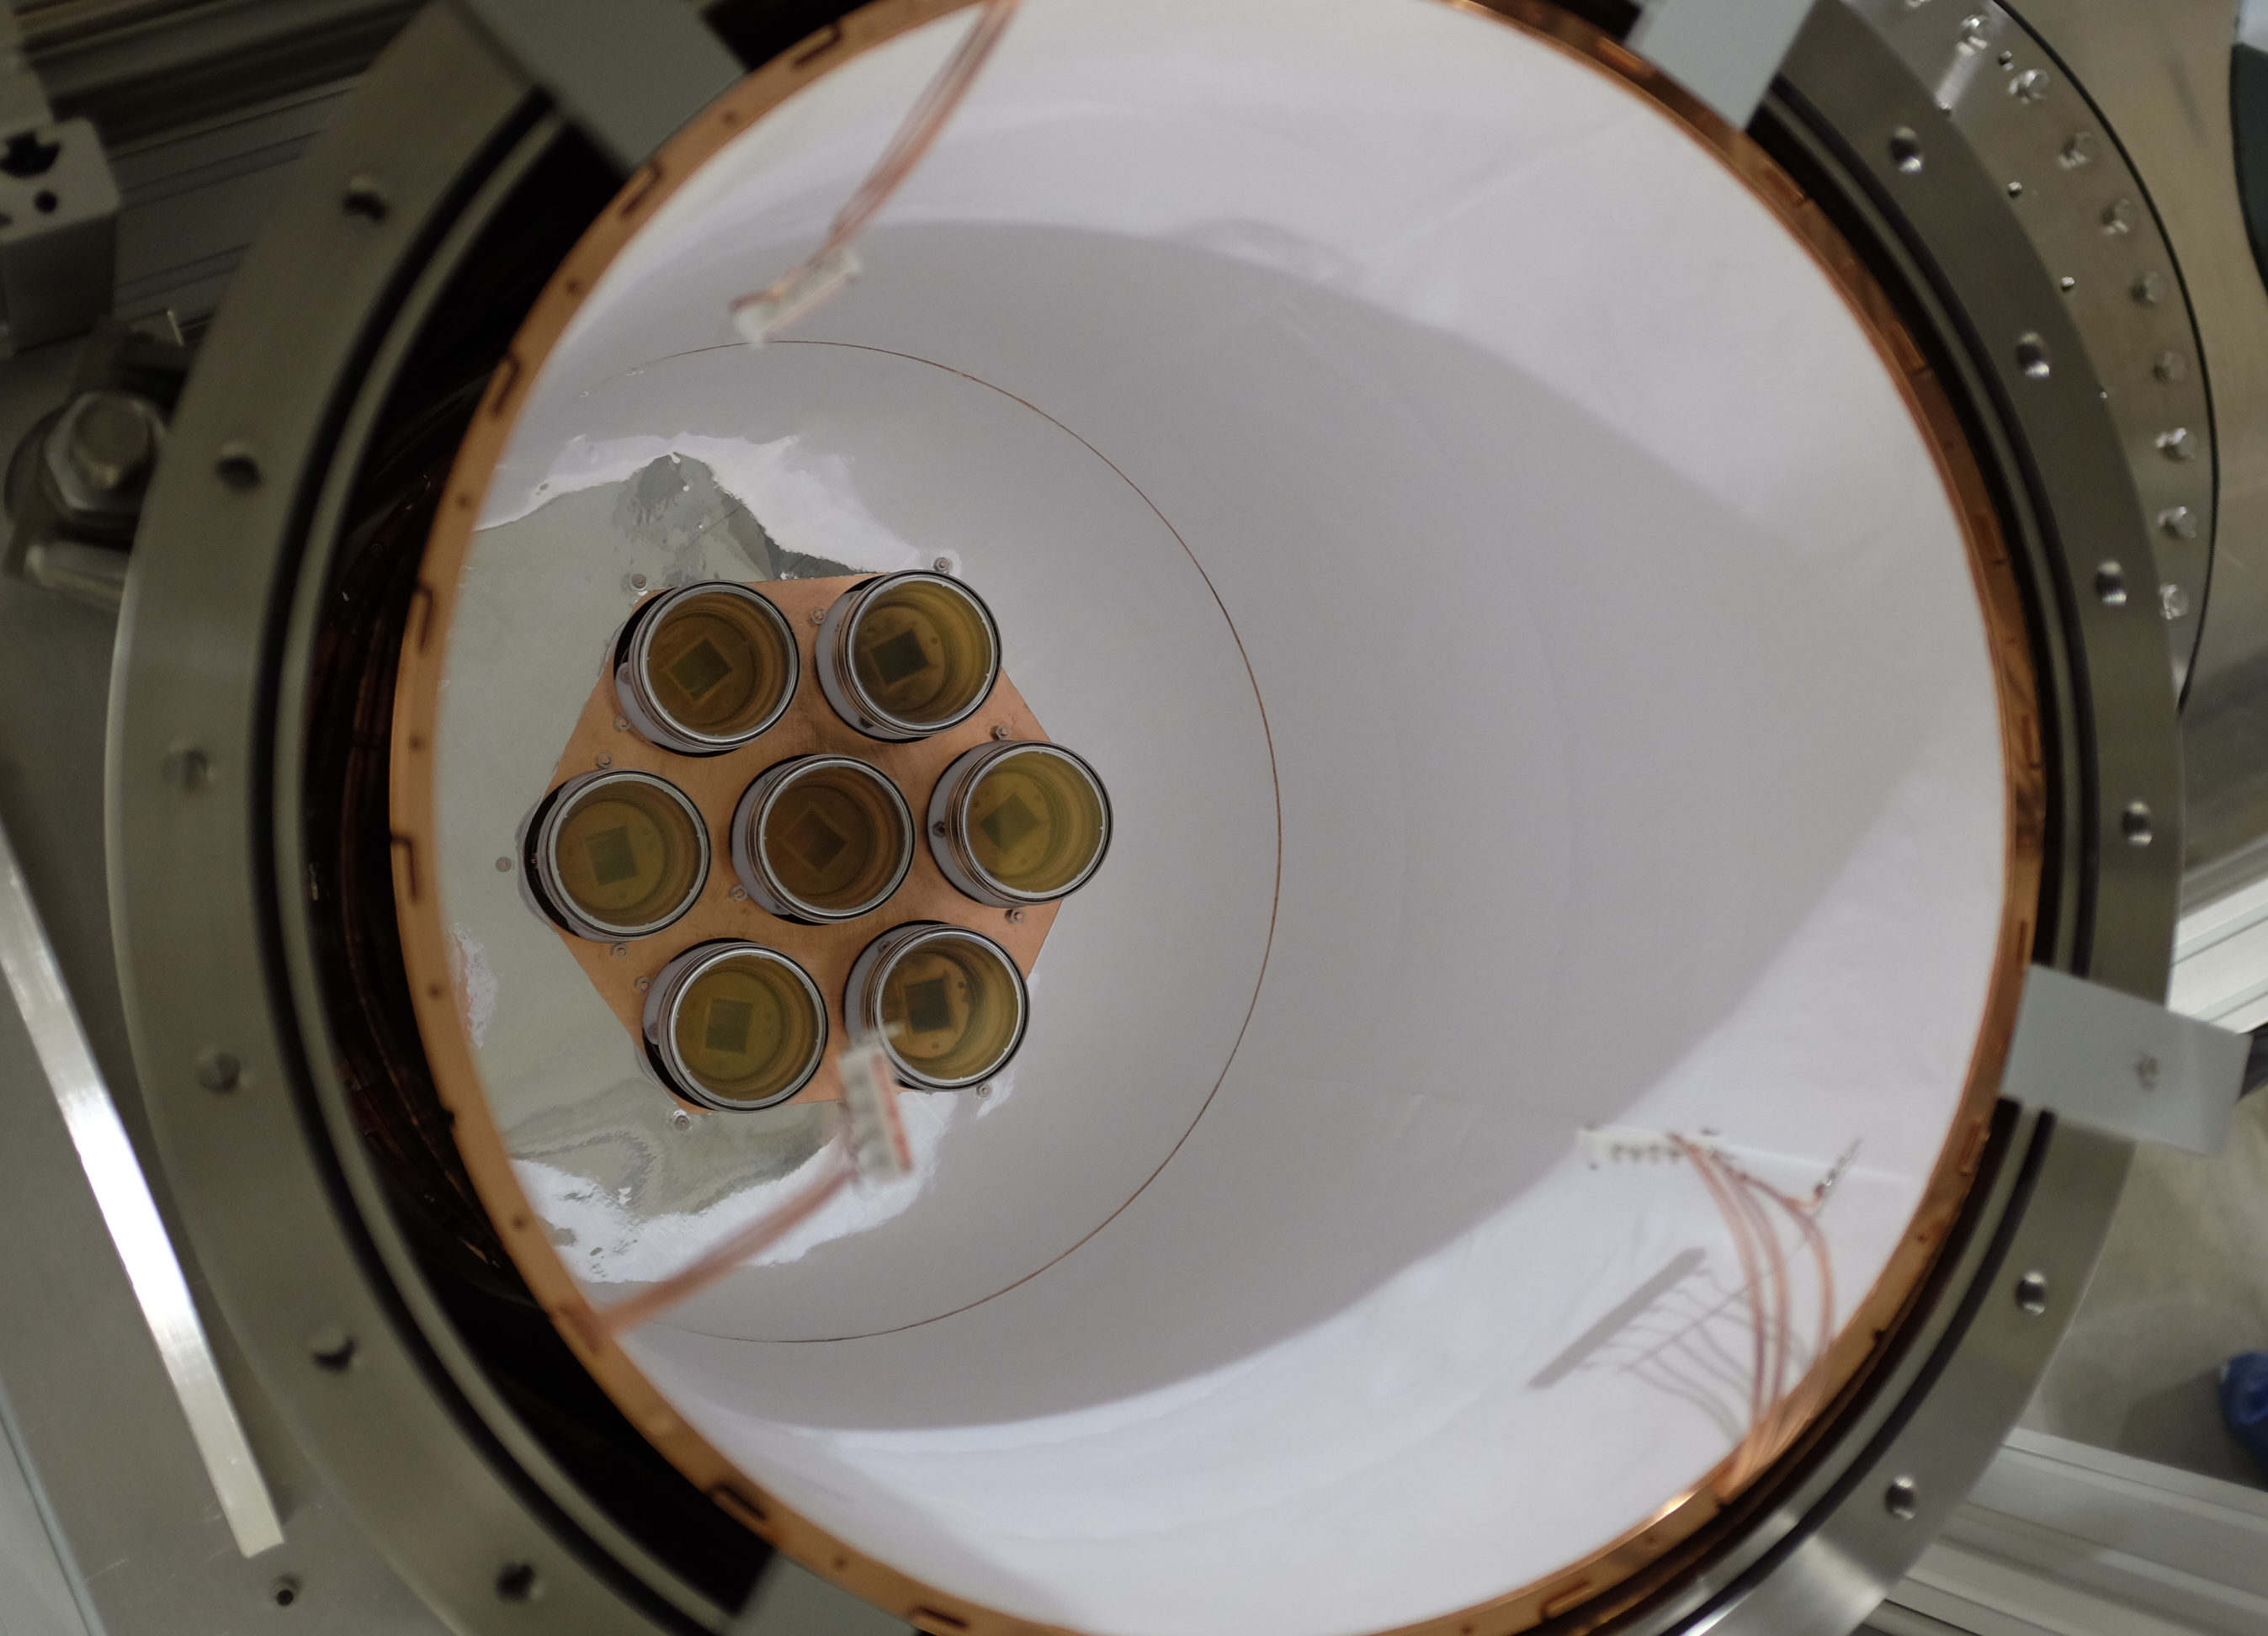
\includegraphics[height=3.7cm]{bottom-pmts.jpg}%%\\%
      % 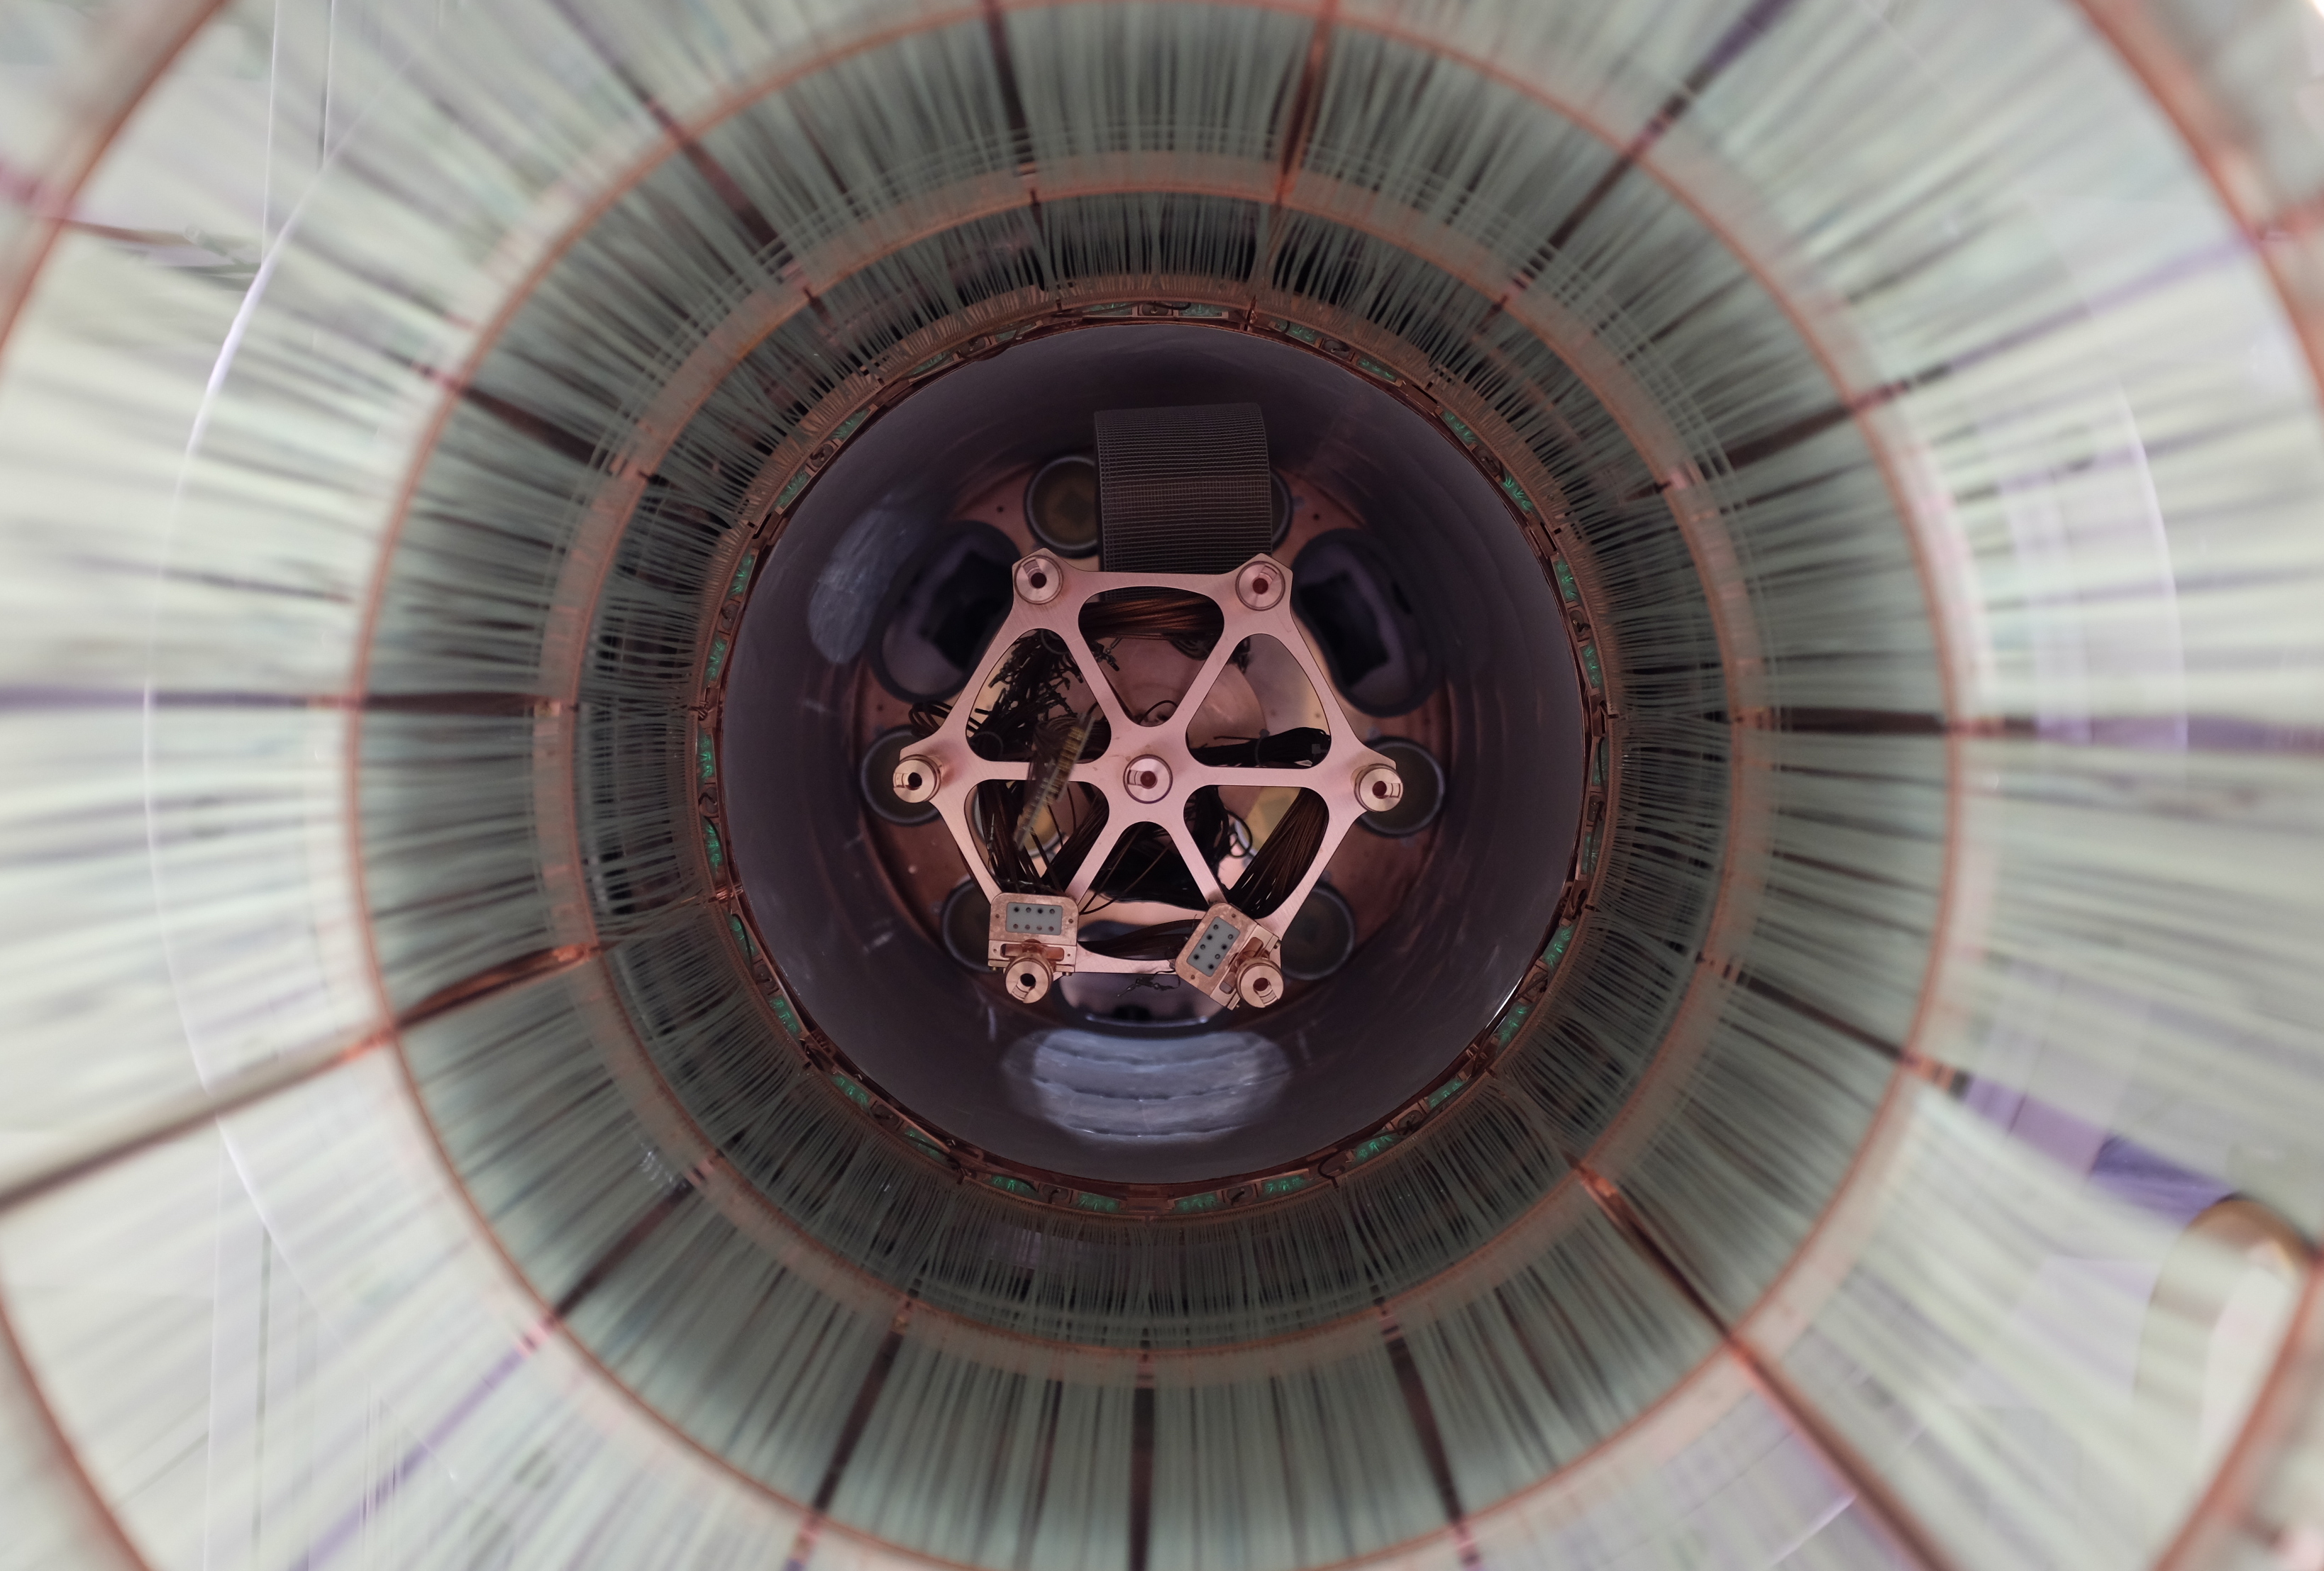
\includegraphics[height=4cm]{setup/fiber-shroud-inside.jpg}%
    };
  \end{tikzpicture}
\end{document}
